\documentclass[]{article}
\usepackage[T1]{fontenc}
\usepackage{lmodern}
\usepackage{amssymb,amsmath}
\usepackage{ifxetex,ifluatex}
\usepackage{fixltx2e} % provides \textsubscript
% Set line spacing
% use upquote if available, for straight quotes in verbatim environments
\IfFileExists{upquote.sty}{\usepackage{upquote}}{}
\ifnum 0\ifxetex 1\fi\ifluatex 1\fi=0 % if pdftex
  \usepackage[utf8]{inputenc}
\else % if luatex or xelatex
  \ifxetex
    \usepackage{mathspec}
    \usepackage{xltxtra,xunicode}
  \else
    \usepackage{fontspec}
  \fi
  \defaultfontfeatures{Mapping=tex-text,Scale=MatchLowercase}
  \newcommand{\euro}{€}
\fi
% use microtype if available
\IfFileExists{microtype.sty}{\usepackage{microtype}}{}
\usepackage[margin=1in]{geometry}
\usepackage{color}
\usepackage{fancyvrb}
\newcommand{\VerbBar}{|}
\newcommand{\VERB}{\Verb[commandchars=\\\{\}]}
\DefineVerbatimEnvironment{Highlighting}{Verbatim}{commandchars=\\\{\}}
% Add ',fontsize=\small' for more characters per line
\usepackage{framed}
\definecolor{shadecolor}{RGB}{248,248,248}
\newenvironment{Shaded}{\begin{snugshade}}{\end{snugshade}}
\newcommand{\KeywordTok}[1]{\textcolor[rgb]{0.13,0.29,0.53}{\textbf{{#1}}}}
\newcommand{\DataTypeTok}[1]{\textcolor[rgb]{0.13,0.29,0.53}{{#1}}}
\newcommand{\DecValTok}[1]{\textcolor[rgb]{0.00,0.00,0.81}{{#1}}}
\newcommand{\BaseNTok}[1]{\textcolor[rgb]{0.00,0.00,0.81}{{#1}}}
\newcommand{\FloatTok}[1]{\textcolor[rgb]{0.00,0.00,0.81}{{#1}}}
\newcommand{\CharTok}[1]{\textcolor[rgb]{0.31,0.60,0.02}{{#1}}}
\newcommand{\StringTok}[1]{\textcolor[rgb]{0.31,0.60,0.02}{{#1}}}
\newcommand{\CommentTok}[1]{\textcolor[rgb]{0.56,0.35,0.01}{\textit{{#1}}}}
\newcommand{\OtherTok}[1]{\textcolor[rgb]{0.56,0.35,0.01}{{#1}}}
\newcommand{\AlertTok}[1]{\textcolor[rgb]{0.94,0.16,0.16}{{#1}}}
\newcommand{\FunctionTok}[1]{\textcolor[rgb]{0.00,0.00,0.00}{{#1}}}
\newcommand{\RegionMarkerTok}[1]{{#1}}
\newcommand{\ErrorTok}[1]{\textbf{{#1}}}
\newcommand{\NormalTok}[1]{{#1}}
\usepackage{graphicx}
% Redefine \includegraphics so that, unless explicit options are
% given, the image width will not exceed the width of the page.
% Images get their normal width if they fit onto the page, but
% are scaled down if they would overflow the margins.
\makeatletter
\def\ScaleIfNeeded{%
  \ifdim\Gin@nat@width>\linewidth
    \linewidth
  \else
    \Gin@nat@width
  \fi
}
\makeatother
\let\Oldincludegraphics\includegraphics
{%
 \catcode`\@=11\relax%
 \gdef\includegraphics{\@ifnextchar[{\Oldincludegraphics}{\Oldincludegraphics[width=\ScaleIfNeeded]}}%
}%
\ifxetex
  \usepackage[setpagesize=false, % page size defined by xetex
              unicode=false, % unicode breaks when used with xetex
              xetex]{hyperref}
\else
  \usepackage[unicode=true]{hyperref}
\fi
\hypersetup{breaklinks=true,
            bookmarks=true,
            pdfauthor={Peter Meißner},
            pdftitle={Studying Public Attention at Election Time},
            colorlinks=true,
            citecolor=blue,
            urlcolor=blue,
            linkcolor=magenta,
            pdfborder={0 0 0}}
\urlstyle{same}  % don't use monospace font for urls
\setlength{\parindent}{0pt}
\setlength{\parskip}{6pt plus 2pt minus 1pt}
\setlength{\emergencystretch}{3em}  % prevent overfull lines
\setcounter{secnumdepth}{0}

%%% Change title format to be more compact
\usepackage{titling}
\setlength{\droptitle}{-2em}
  \title{Studying Public Attention at Election Time}
  \pretitle{\vspace{\droptitle}\centering\huge}
  \posttitle{\par}
  \author{Peter Meißner}
  \preauthor{\centering\large\emph}
  \postauthor{\par}
  \predate{\centering\large\emph}
  \postdate{\par}
  \date{2014-12-03}




\begin{document}

\maketitle


\subsection{Intro}\label{intro}

Elections are major political events and their results determine who
gets to be in governemnt for the next view years. But how long do
elections and their results capture the public's attention. Let us have
a look at Wikipedia page access statistics to find out.

Our weapon of choice will be \emph{R} and the newly published
\emph{wikipediatrend} package that allows for convenient data retreival
-- have a look here
\href{http://cran.r-project.org/web/packages/wikipediatrend/index.html}{wikipediatrend
on CRAN} and especially here
\href{https://github.com/petermeissner/wikipediatrend}{wikipediatrend on
GitHub} for more information on the package.

As running example we rely on national elections in Germany covered by
the \href{http://de.wikipedia.org/wiki/Bundestagswahl}{German Wikipedia
article \emph{Bundestagswahl}}. Since late 2007 (the first time data is
available) Germany had two elections at national level -- one in
September of 2009 and one in September 2013 -- both resulting in
governments led by
\href{http://en.wikipedia.org/wiki/Angela_Merkel}{Angela Merkel}.

\subsection{Getting data and having a first
glance}\label{getting-data-and-having-a-first-glance}

First, we load the \emph{wikipediatrend} package that will help fetching
the data:

\begin{Shaded}
\begin{Highlighting}[]
\KeywordTok{require}\NormalTok{(wikipediatrend)}
\end{Highlighting}
\end{Shaded}

Next, we use \texttt{wp\_trend()} to download the data and save it into
\texttt{bt\_election}. Within \texttt{wp\_trend()} we use
\texttt{page = "Bundestagswahl"} to get counts for the overview article.
Furthermore, we specify \texttt{2007-01-01} in format
\texttt{yyyy-mm-dd} as \texttt{from} date, \texttt{de} to get the German
language flavor of Wikipedia, \texttt{friendly = T} to ensure automatic
saving and reuse of downloaded data as well as \texttt{userAgent = T} to
tell the server that the data is requested by an R user with
wikipediatrend package: wikipediatrend running on: x86\_64-w64-mingw32 ,
R version 3.1.2 (2014-10-31).

\begin{Shaded}
\begin{Highlighting}[]
\NormalTok{bt_election <-}\StringTok{ }\KeywordTok{wp_trend}\NormalTok{(  }\DataTypeTok{page      =} \StringTok{"Bundestagswahl"}\NormalTok{, }
                          \DataTypeTok{from      =} \StringTok{"2007-01-01"}\NormalTok{, }
                          \DataTypeTok{lang      =} \StringTok{"de"}\NormalTok{, }
                          \DataTypeTok{friendly  =} \NormalTok{T,}
                          \DataTypeTok{userAgent =} \NormalTok{T)}
\NormalTok{bt_election <-}\StringTok{ }\NormalTok{bt_election[ }\KeywordTok{order}\NormalTok{(bt_election$date), ]}
\end{Highlighting}
\end{Shaded}

We managed to get 2531 data points:

\begin{Shaded}
\begin{Highlighting}[]
\KeywordTok{dim}\NormalTok{(bt_election)}
\end{Highlighting}
\end{Shaded}

\begin{verbatim}
## [1] 2531    2
\end{verbatim}

\ldots{} in between 2007-12-10 and 2014-12-04

\begin{Shaded}
\begin{Highlighting}[]
\KeywordTok{summary}\NormalTok{(bt_election$date)}
\end{Highlighting}
\end{Shaded}

\begin{verbatim}
##         Min.      1st Qu.       Median         Mean      3rd Qu.         Max. 
## "2007-12-10" "2009-09-23" "2011-06-18" "2011-06-16" "2013-03-11" "2014-12-04"
\end{verbatim}

\ldots{} looking like that:

\begin{Shaded}
\begin{Highlighting}[]
\NormalTok{bt_election[}\DecValTok{55}\NormalTok{:}\DecValTok{60}\NormalTok{, ]}
\end{Highlighting}
\end{Shaded}

\begin{verbatim}
##          date count
## 55 2008-02-03   349
## 56 2008-02-04   481
## 57 2008-02-05   584
## 58 2008-02-06   668
## 59 2008-02-07   566
## 60 2008-02-08   351
\end{verbatim}

\begin{Shaded}
\begin{Highlighting}[]
\KeywordTok{plot}\NormalTok{(bt_election, }\DataTypeTok{type=}\StringTok{"h"}\NormalTok{, }\DataTypeTok{ylim=}\KeywordTok{c}\NormalTok{(-}\DecValTok{1000}\NormalTok{,}\DecValTok{40000}\NormalTok{))}
\end{Highlighting}
\end{Shaded}

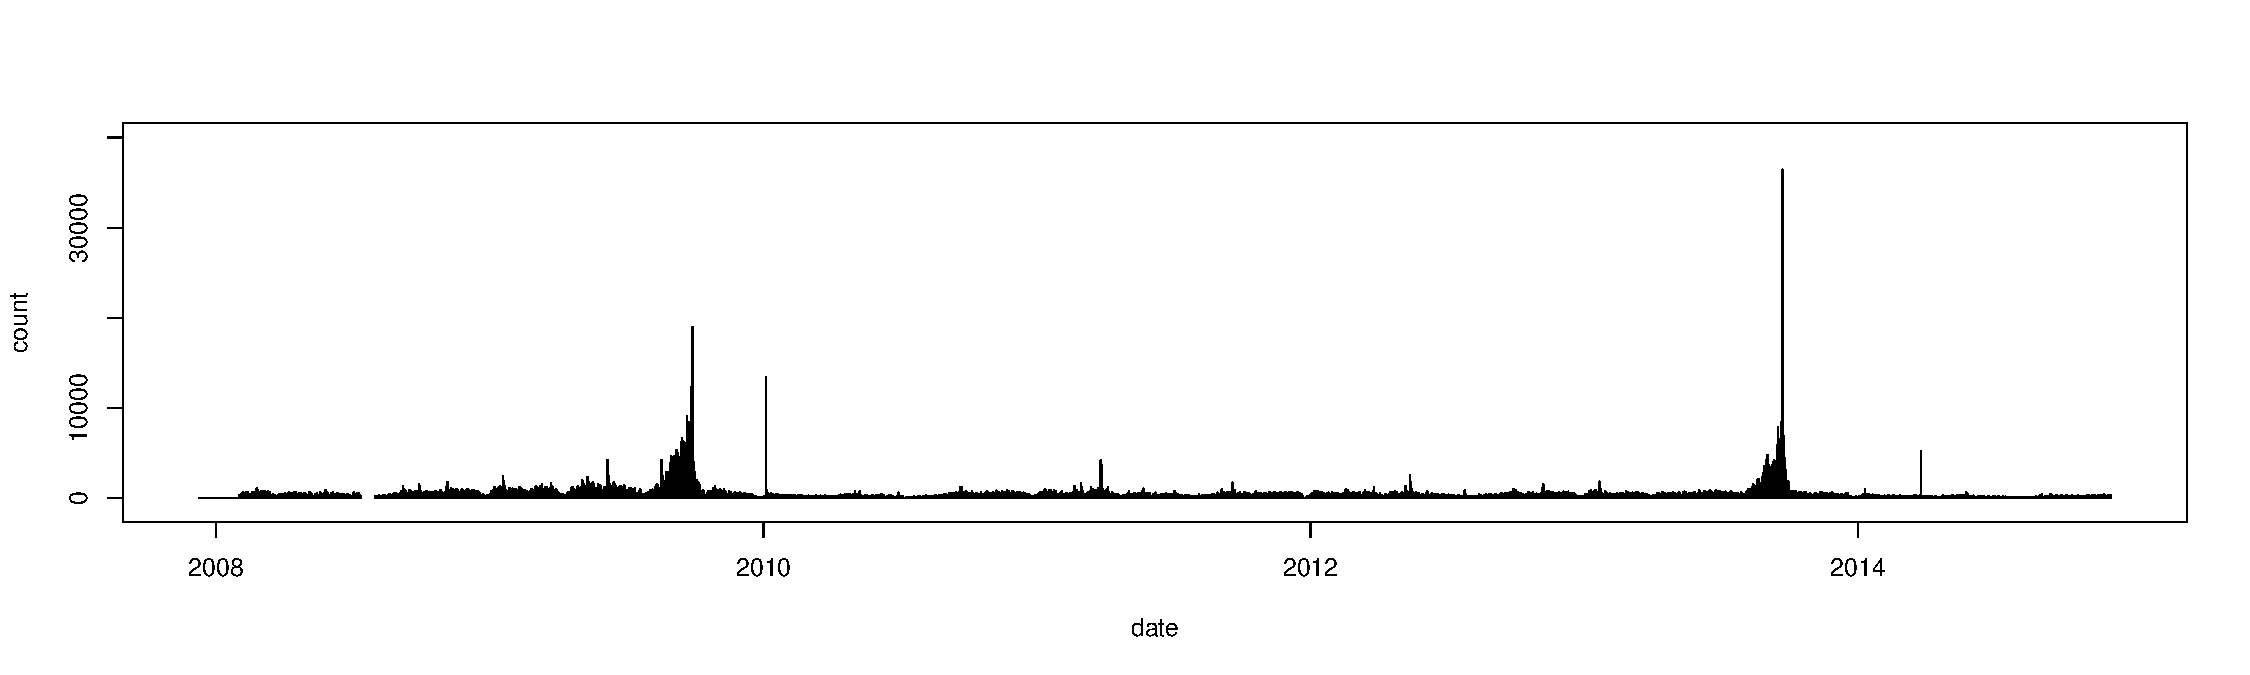
\includegraphics{wikipediatrendblog_files/figure-latex/unnamed-chunk-4-1.pdf}

The public attention the Wikipedia article got peaks well above 35,000
views per day and overall we can find two distinct bulks of attention
each in late 2009 and 2013.

\subsection{Tweaking the plot}\label{tweaking-the-plot}

Let put some more effort into the visualization by splitting our counts
into normals (lower 95\% of the values) and those being unusual large
(upper 5\% of the values).

\begin{Shaded}
\begin{Highlighting}[]
\NormalTok{count_big       <-}\StringTok{ }\NormalTok{bt_election$count >}\StringTok{ }\KeywordTok{quantile}\NormalTok{(bt_election$count, }\FloatTok{0.95}\NormalTok{)}
\NormalTok{count_big_col   <-}\StringTok{ }\KeywordTok{ifelse}\NormalTok{(count_big, }\StringTok{"red"}\NormalTok{, }\StringTok{"black"}\NormalTok{)}
\end{Highlighting}
\end{Shaded}

The following plot than visualizes page access counts for the Wikipedia
article \emph{Bundestagswahl} from the German Wikipedia on a daily basis
with red bars for upper 5\% of the values and black bars for the other
95\%. The triangles pointing at the bars from above mark the two
election dates -- 27th of September in 2009 and 22nd of September in
2013 -- that occurred during the time span under observation.

\begin{Shaded}
\begin{Highlighting}[]
\KeywordTok{plot}\NormalTok{(bt_election, }\DataTypeTok{type=}\StringTok{"h"}\NormalTok{, }\DataTypeTok{col=}\NormalTok{count_big_col, }\DataTypeTok{ylim=}\KeywordTok{c}\NormalTok{(-}\DecValTok{1000}\NormalTok{,}\DecValTok{40000}\NormalTok{))}
\KeywordTok{arrows}\NormalTok{( }\DataTypeTok{x0  =} \KeywordTok{as.numeric}\NormalTok{(}\KeywordTok{c}\NormalTok{(}\KeywordTok{wp_date}\NormalTok{(}\StringTok{"2013-09-22"}\NormalTok{),}\KeywordTok{wp_date}\NormalTok{(}\StringTok{"2009-09-27"}\NormalTok{))),}
        \DataTypeTok{x1  =} \KeywordTok{as.numeric}\NormalTok{(}\KeywordTok{c}\NormalTok{(}\KeywordTok{wp_date}\NormalTok{(}\StringTok{"2013-09-22"}\NormalTok{),}\KeywordTok{wp_date}\NormalTok{(}\StringTok{"2009-09-27"}\NormalTok{))),}
        \DataTypeTok{y0  =} \DecValTok{40000}\NormalTok{, }\DataTypeTok{y1  =} \DecValTok{39500}\NormalTok{, }\DataTypeTok{lwd =} \DecValTok{3}\NormalTok{, }\DataTypeTok{col=}\StringTok{"red"}\NormalTok{)}
\KeywordTok{legend}\NormalTok{(}\DataTypeTok{x=}\StringTok{"topleft"}\NormalTok{, }\DataTypeTok{col=}\KeywordTok{c}\NormalTok{(}\StringTok{"red"}\NormalTok{, }\StringTok{"black"}\NormalTok{), }\DataTypeTok{legend=}\KeywordTok{c}\NormalTok{(}\StringTok{"upper 5% quantile"}\NormalTok{, }\StringTok{"lower 95% quantile"}\NormalTok{), }\DataTypeTok{lwd=}\DecValTok{1}\NormalTok{)}
\end{Highlighting}
\end{Shaded}

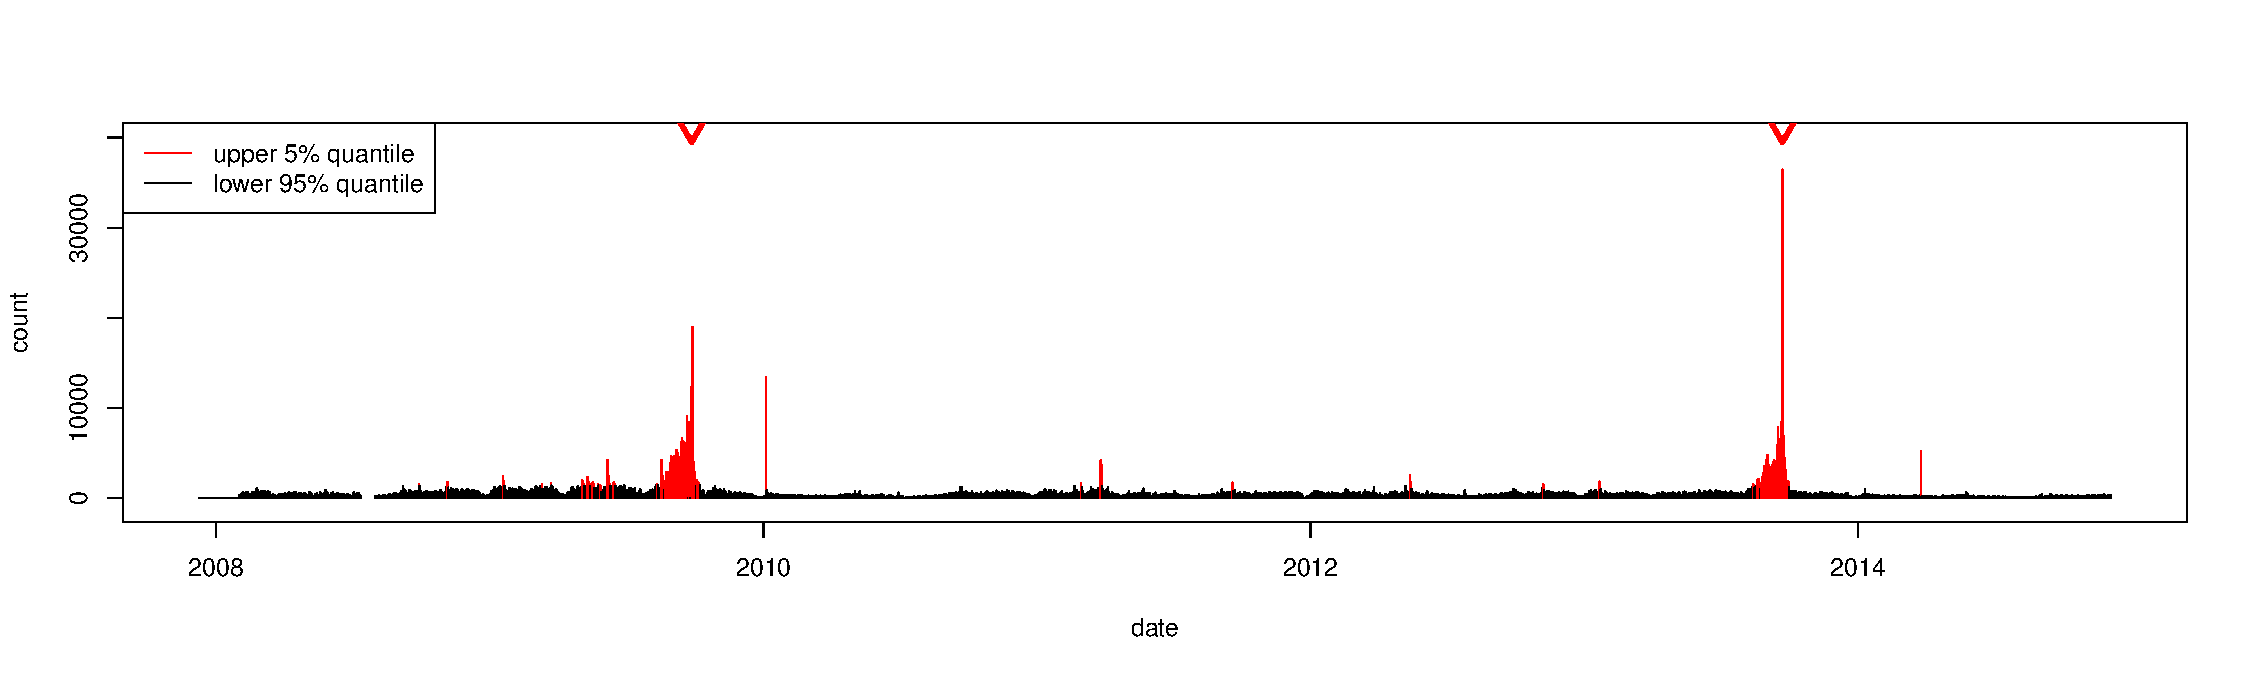
\includegraphics{wikipediatrendblog_files/figure-latex/plotting_data-1.pdf}

Adding the election date to the graph reveals that the article's public
attention imeadatly falls back to normal after the election has taken
place. Obviously the highten puplic attention does not stem from people
informing themselves after the the election has taken place about its
results leaving us with the puzzle, why else they should use the page.
Maybe the attention stems from the need to understand what is going on
at election day and which of the two votes goes directly to the
candidate and which of the two is for the party.

\subsection{Credits}\label{credits}

As far as I know we have to thank Domas Mituzas and User:Henrik for the
API provided at \href{http://stats.grok.se/}{stats.grok.se} --
\href{http://stats.grok.se/about}{see here}.

\end{document}
